\documentclass[a4paper,12pt]{article}

\usepackage{cmap}		
\usepackage[utf8]{inputenc}			
\usepackage[english,russian]{babel}
\usepackage{framed}
\usepackage{hyperref}
\usepackage{amsmath}
\usepackage{graphicx}
\usepackage[colorinlistoftodos]{todonotes}
\usepackage{wrapfig}
\usepackage{lipsum}
\usepackage{listings}
\usepackage{color}
\usepackage{indentfirst}
\usepackage{times}
\usepackage{textcomp}
\usepackage{xcolor}
\usepackage{tabu}
\usepackage{colortbl}
\usepackage{minted}
\usepackage{xcolor}
\usepackage{listings}
\usepackage{smartdiagram}
\usepackage{xcolor}
\usepackage{gensymb}
\usepackage{siunitx}
\usepackage{tikz}
\usetikzlibrary{shapes,arrows}
\usepackage{lscape}
\newcommand{\HRule}{\rule{\linewidth}{0.5mm}}
\usepackage[T1]{fontenc}
\usepackage{bigfoot} % to allow verbatim in footnote
\usepackage[numbered,framed]{matlab-prettifier}

\usepackage{filecontents}
\begin{filecontents*}{ai.m}
s=tf('s');
ss_motor=0.772/(0.000103*s^3+0.103*s^2+s)
figure(); bode(ss_motor); title ("Motor");
ss_compensator=(136.85*(1+0.00035*s)*(1+0.018*s))/(1+0.0012*s)
ss_after_compensating=ss_motor*ss_compensator;
figure(); bode(ss_after_compensating); title ("After compensating");
ss_feedback=ss_after_compensating/(1+ss_after_compensating)
figure(); bode(ss_feedback) ;title ("closed loop");
figure(); step(ss_feedback,t); title ("step response");
t=0:0.01:10;
u=(2*pi/3)*sin(0.628*t);
g=lsim(ss_feedback,u,t);
figure(); plot(t,(g'-u)*180/pi); title ("The error for a sinewave input signal");
%controlSystemDesigner('bode',ss_motor)
\end{filecontents*}


\let\ph\mlplaceholder % shorter macro
\lstMakeShortInline"

\lstset{
  style              = Matlab-editor,
  basicstyle         = \mlttfamily,
  escapechar         = ",
  mlshowsectionrules = true,
}

\begin{document}

\begin{titlepage}
\begin{center}

\textsc{\Large Московский Государственный Технический Университет имени Н.Э.Баумана}\\
\textsc{\large (Национальный Исследовательский Университет)}\\[1.5cm]

% Upper part of the page. The '~' is needed because \\
% only works if a paragraph has started.

\includegraphics[width=0.3\textwidth]{img/logo.png}~\\[1cm]

\textsc{\Large Домашнее задание №1 по \\ Интеллектуаьные системы в мехатронике и робототехнике}\\[0.5cm]

% Title
\HRule \\[0.4cm]
{ \LARGE \bfseries  моделирование и анализ системы управления двигателя\\ [0.4cm] }

\HRule \\[1.5cm]

% Author and supervisor
\noindent
\begin{minipage}{0.4\textwidth}
\begin{flushleft} \large
\emph{Студенты:}\\
Юнес \textsc{А.}\\
Али  \textsc{З.}\\
Цюй \textsc{K.}
\end{flushleft}
\end{minipage}%
\begin{minipage}{0.4\textwidth}
\begin{flushright} \large
\emph{Преподаватель:} \\
Бщшляков \textsc{А.~А.}
\end{flushright}
\end{minipage}

\vfill

% Bottom of the page
{\large \today}

\end{center}
\end{titlepage}

\newpage
\tableofcontents
\newpage
\listoffigures
\newpage
\section{Постановка задачи}
Лабораторный стенд, представляющий собой электропривод, в котором известна силовая часть. \\
Требуется:\\
Синтезировать и реализовать систему управления электроприводом постоянного тока, отвечающую следующим условиям:\\
На вход системы поступает сигнал следующего вида: $g(t)=g_m sin(\omega t)$\\
где $g_m =120\degree$, $\omega=0,1$ Гц $= 0,628$ рад/с\\
Ошибка системы: $\Delta \varepsilon=60'=1\degree$\\
При наличии ступенчатого управляющего воздействия $g(t) = 1(t)$ \\
перерегулирования $\sigma = 30\%$\\

Технические характеристики двигателя:\\
Номинальное напряжения $U_n=27 $ B\\
Номинальная частота вращения $N_n=2500 $ об/мин$=261.80$рад/с\\
Номинальный ток $I_n=0.15 $ A\\
Номинальный момент $M_n = 50$ Г*см $= 5*10^{-3}$ Н*м\\
Электрическая постоянная $T_e = 0.6 - 1$ мс $ = (0.6 - 1)*10^{-3} $ с\\
Электромеханическая постоянная $T_m =0.035 - 0.05$ с\\
Сопротивление обмоток якоря $R_{a}=107 $ ом\\
Коэффициент полезного действия $\eta=69 \%$\\
Момент инерции якоря $J_{a} = 1,16* 10^{-6} $ кг*м$^2$\\

Габаритные размеры двигателя:\\
Длина: $L=50 $ мм\\
Диаметр: $d=20$ мм\\
Масса: $m=0.25$ кг\\

Нагрузка\\
$m = 1 $кг - масса груза\\
$R = 5.5*10^{-3} $м – радиус блока \\

Редуктор:\\
i = 133 – передаточное число редуктора.

\newpage
\section{ Математическая модель}
Система уравнений динамики для двигателя постоянного тока:
$$U(t)=R.I(t)+L.\frac{dI(t)}{dt}+k_\omega \frac{d\alpha(t)}{dt}$$
$$M(t)=k_m.I(t)=J_\varepsilon \frac{d^2 \alpha(t)}{dt^2}$$

После преоброзования Лапласа:
$$U(s)=R.I(s)+L.s.I(s)+k_\omega .s.\alpha(s)$$
$$\Rightarrow U(s)-k_\omega.s.\alpha=I(s)(R+L.s)$$
$$\Rightarrow \frac{I(s)}{U(s)-k_\omega.s.\alpha(s)}=\frac{1}{R+L.s}$$
$$M(s)=k_m.I(s)\Rightarrow \frac{M(s)}{I(s)}=k_m$$
$$M(s)=J_\varepsilon.s^2.\alpha(s)\Rightarrow\frac{s^2.\alpha(s)}{M(s)}=\frac{1}{J_\varepsilon}$$
На основе этих уравнений была собрана модель двигателя:
\\

\tikzstyle{block} = [draw, rectangle, 
    minimum height=3em, minimum width=6em]
\tikzstyle{var}=[draw,rectangle,minimum height=3em,minimum width=3em]
\tikzstyle{sum} = [draw, circle, node distance=1cm]
\tikzstyle{input} = [coordinate]
\tikzstyle{output} = [coordinate]
\tikzstyle{pinstyle} = [pin edge={to-,thin,black}]

% The block diagram code is probably more verbose than necessary
\begin{figure}[h]
    \centering
    \begin{tikzpicture}[auto, node distance=3cm,>=latex']
    % We start by placing the blocks
    \node [input, name=input] {};
    \node [sum, right of=input] (sum) {};
    \node [block, right of=sum,node distance=2cm] (frac) {\large $\frac{1}{R+L.s}$};
    \node [var, right of=frac] (km) {\large $k_m$};
    \node [var, right of= km,,node distance=2.5cm] (j) {\large $\frac{1}{J_\varepsilon}$};
    \node [var,right of =j,node distance=2.5cm] (s_1) {\large $\frac{1}{s}$};
    \node [output, right of=s_1,node distance=2cm] (output) {};
    \draw [->] (km) -- node [name=m]{$M(s)$} (j);
    \node [var , below of= m] (kw){\large $k_\omega$};
    
    % Once the nodes are placed, connecting them is easy. 
    \draw [draw,->] (input) -- node {$U(s)$} (sum);
    \draw [->] (sum) -- node {} (frac);
    \draw [->] (frac) -- node {$I(s)$} (km);
    \draw [->] (j) -- node {$\ddot{\alpha}(s)$} (s_1);
    \draw [->] (s_1) -- node [name=y] {$\dot{\alpha}(s)$}(output);
    \draw [->] (y) |- (kw);
    \draw [->] (kw) -| node[pos=0.99] {$-$} node [near end] {} (sum);
\end{tikzpicture}
    \caption{Структурная схема двигателя постоянного тока}
    \label{fig:my_label}
\end{figure}

Передаточная функция двигателя:
$$W(s)=\frac{k_m}{j_\varepsilon.s.(R+Ls)}$$
$$\frac{\dot{\alpha(s)}}{U(s)}=\frac{W(s)}{1+W(s)k_\omega}=\frac{k_m}{j_\varepsilon.s.(R+Ls)+k_m.k_\omega}=\frac{\frac{1}{k_w}}{T_e.T_m.s^2+T_m.s+1}$$
\newpage
Постоянная ЭДС:
$$k_\omega =\frac{U_n-R_a.I_n}{\omega_n}=\frac{27-107*0.15}{261.8}=0.0418 V.s.rad^{-1}\Rightarrow \frac{1}{k_\omega}=23.9$$
Электрическая постоянная : $T_e=0.001 s$\\
Электромеханическая постоянная без нагрузки: $T_m=0.05 s$\\
Передаточная функция двигателя без нагрузки:
$$ \frac{\dot{\alpha(s)}}{U(s)}= \frac{23.9}{0,00005s^2+0,05s+1}$$
Электромеханическая постоянная с нагрузкой: 
$$K_m=\frac{M_n}{I_n}=\frac{0.005}{0.15}=0.033$$
$$J=J_a+J_{red}+\frac{J_l}{i_red^2}=1.15J_a+\frac{m.r^2}{2.i^2}=1.15*1.16*10^{-6}+\frac{5.5^2*10^{-6}}{2*133^2}=1.3348*10^{-6}$$
$$T'_m=\frac{J.R_a}{k_m.k_\omega}=\frac{1.3348*10^{-6}*107}{0.033*0.0418}=0.103s$$
Передаточная функция двигателя с нагрузкой:
$$W(s)=\frac{\dot{\alpha(s)}}{U(s)}= \frac{23.9}{0.000103s^2+0,103s+1}$$
Для построения польная система, нужно добавить:
\begin{itemize}
    \item Интегратор $\frac{1}{s}$ на выходы двигатля чтобы получить углу.
    \item Коэффициент редуктора $k_{red}=\frac{1}{i}$ чтобы преоброзовать выходной угол двигателя в выходной угол вала привод.
    \item Коэффициент датчика $k_{sensor}=\frac{3}{2\pi}$ переводит значение угла в напряжени (диапазон напряжени датчика 0-3 В).
    \item Коэффициент АЦП $k_{ADC}=\frac{4096}{3}$ переводит напряжение в число диапазоне [0, 4095].
    \item Коэффициент ШИМ $k_{PWM}=\frac{8400}{4096}$  преобразует число, полученное АЦП МК в число коэффициентa ШИМ (16 биты $\Rightarrow$ 8400 уровни).
    \item Коэффициент ЦАП $k_{DAC}=\frac{3}{8400}$.
    \item Коэффициент усилителя мощности $k_{op_amp}=\frac{27}{3}$
    \item Коэффициент генератора сигналов $k_{gen}=\frac{3}{360}$ переводит значение угла в напряжени (диапазон напряжени датчика 0-3 В).
\end{itemize}
\begin{landscape}
Полбный модель системы управления:
% The block diagram code is probably more verbose than necessary
\begin{figure}[h]
    \centering
    \begin{tikzpicture}[auto, node distance=3cm,>=latex']
    % We start by placing the blocks
    \node [input, name=input] {};
    \node [var, right of= input,node distance=1.5cm] (gen) {\large $k_{gen}$};
    \node [sum, right of=gen,node distance=1.5cm] (sum) {};
    \node [var, right of= sum,node distance=1.5cm] (adc) {\large $k_{ADC}$};
    \node [var, right of= adc,node distance=2cm] (pwm) {\large $k_{PWM}$};
    \node [var, right of= pwm,node distance=2cm] (dac) {\large $k_{DAC}$};
    \node [var, right of= dac,node distance=2cm] (op) {\large $k_{op_amp}$};
    \node [block, right of=op,node distance=2.5cm] (motor) {\large Двигатель};
    \node [var, right of=motor,node distance=2.5cm] (km) {\large $\frac{1}{s}$};
    \node [var, right of= km,node distance=2cm] (red) {\large $k_{red}$};
    \node [var, right of= red,node distance=2cm] (sensor) {\large $k_{sensor}$};
    \node [output, right of=sensor,node distance=2cm] (output) {};
    \draw [->] (op) -- node [name=m]{} (motor);
    \node [var , below of= m] (kw){\large 1};
    
    % Once the nodes are placed, connecting them is easy. 
    \draw [->] (input) -- node {} (gen);
    \draw [->] (gen) --node {} (sum);
    \draw [->] (sum) -- node {} (adc);
    \draw [->] (adc) -- node {} (pwm);
    \draw [->] (pwm) -- node {} (dac);
    \draw [->] (dac) -- node {} (op);
    \draw [->] (motor) -- node {} (km);
    \draw [->] (km) -- node {} (red);
    \draw [->] (red) -- node {} (sensor);
    \draw [->] (sensor) -- node [name=y] {$V_out(s)$}(output);
    \draw [->] (y) |- (kw);
    \draw [->] (kw) -| node[pos=0.99] {$-$} node [near end] {} (sum);
\end{tikzpicture}
    \caption{Структурная схема системы управления}
    \label{fig:my_label}
\end{figure}

Коэффициент усиления прямой цепи:\\
$$K=k_{red}*k_{sensor}*k_{ADC}*k_{PWM}*k_{DAC}*k_{op_amp}=\frac{1}{133}.\frac{3}{6.28}.\frac{4096}{3}.\frac{8400}{4096}.\frac{3}{8400}.\frac{27}{3}=0.0323$$
Передаточная функция системы:\\
$$W'(s)=\frac{V_out(s)}{V_signal(s)}=\frac{W(s)\frac{K}{s}}{1+W(s)\frac{K}{s}}=\frac{0.772}{0.000103s^3+0.103s^2+s+0.772}$$
\end{landscape}
\newpage
\section{Определения критерии проектерования}
\begin{itemize}
    \item Рабочая точка: точка выше которой должна проходить ЛАЧХ разомкнутой системы, чтобы удовлетворять требованиям по точности. Начинаем с передаьочная функция ошибка, получим:
    $$\Phi_\varepsilon(s)=\frac{E(s)}{G_in(s)}=\frac{1}{1+W(s)}$$
    В области низких частот, $W(s)>>1$ (смотри рис.3):
    $$\Phi_\varepsilon(s)=\frac{E(s)}{G_in(s)}=\frac{1}{W(s)}$$
    $$\Rightarrow |W(s)|=\frac{|G_in(s)|}{|E(s)|}$$
    Рабочая частота: $\omega_work=0.628 rad/s$\\
    Значения амплитуды:
    $$20log(|W(s)|)+3dB=20log(\frac{|G_in(s)|}{|E(s)|})+3dB=$$
    $$=20log(\frac{g_m}{\Delta \varepsilon})+3dB=20log(\frac{120}{1})+3dB=44.85dB$$
    \item перерегулирования $\sigma = 30\%$\\
\end{itemize}
Рассмотрим Рис.3 (нескорректированная система), можем наблюдать:
\begin{itemize}
    \item Запас устойчивости по фазе: 85,5\degree
    \item Запас устойчивости по амплитуде: 62.2 dB
    \item Амплитуда на рабочая чатота $\ne$ 44,85 dB
    \item Cистема является устойчивой и удовлетворяет требованиям по перерегулированию, но не удовлетворяет требованиям по ошибке. 
\end{itemize}
\newpage
\begin{landscape}
\begin{figure}[h]
    \centering
    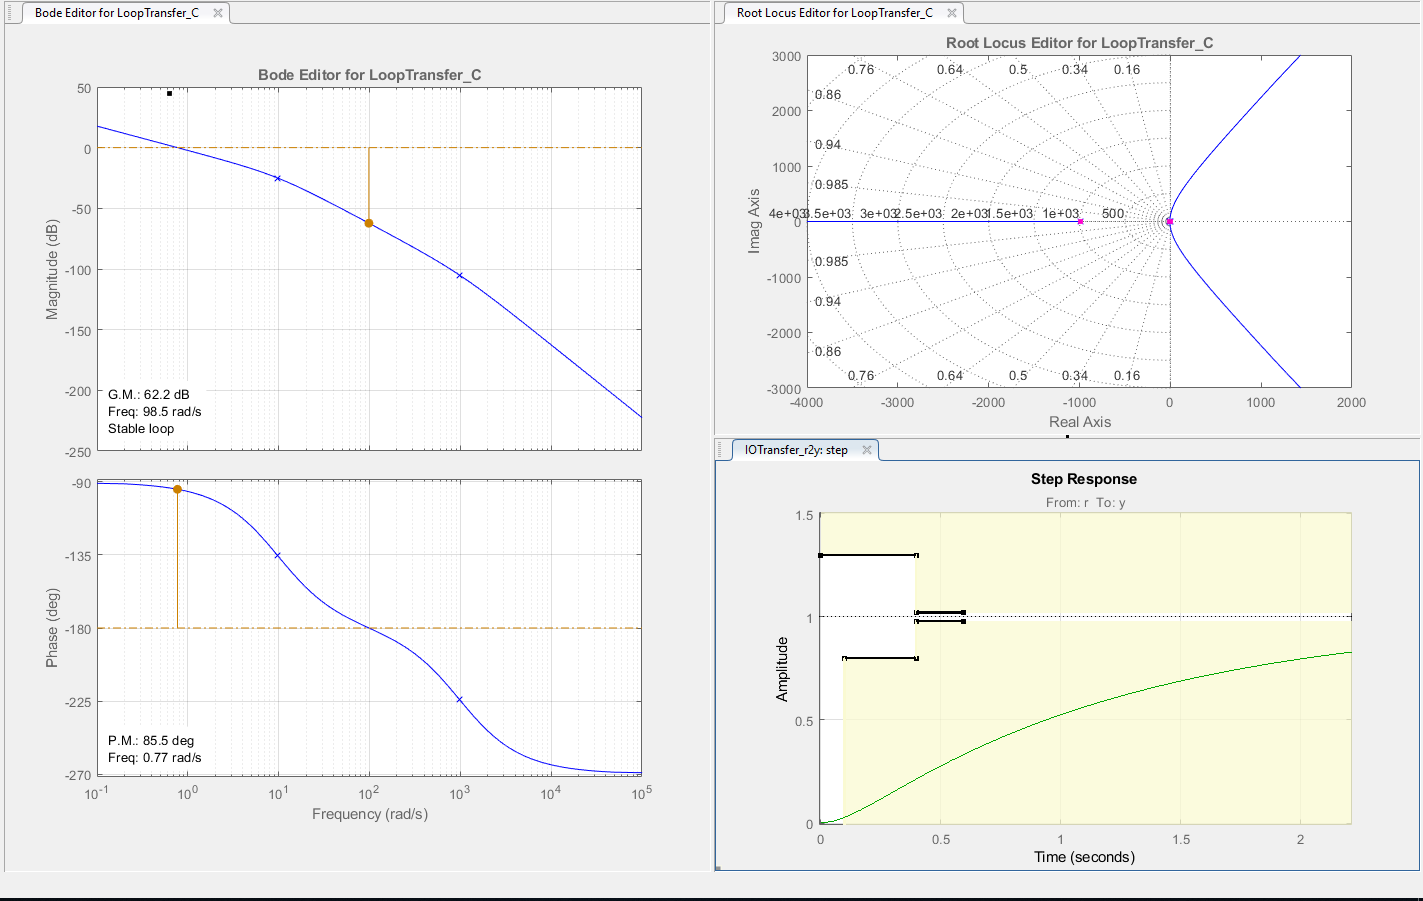
\includegraphics[height=15cm]{img/uncompensated.PNG}
    \caption{ЛАЧХ, ЛФЧХ, коренвой годораф нескорректированная система}
    \label{fig:my_label}
\end{figure}
\end{landscape}
\section{Проектерования системы управления}
Чтобы получить желаемые результаты, нам нужно добавить корректерующее звено.\\
Определения полюсы и нули корректерующего звена, мы использовали controlSystemDesigner в Matlab.\\
Мы получим лучшие резудтаты по использованию компенсатор со следующими свойствами:
\begin{itemize}
    \item Коэффицинт уселения = 136,85
    \item Нули в точках : -2840 , -55,5
    \item Полюс в точки : -863
    \item Передаточная функция компенсатора:
    $$C(s)=136.85\frac{(1+0.00035s)(1+0.018s)}{(1+0.0012s)}$$
    $$C(s)=\frac{0.0008622 s^2+2.511 s + 136.8}{0.0012 s+1}$$
\end{itemize}
\begin{figure}[h]
    \centering
    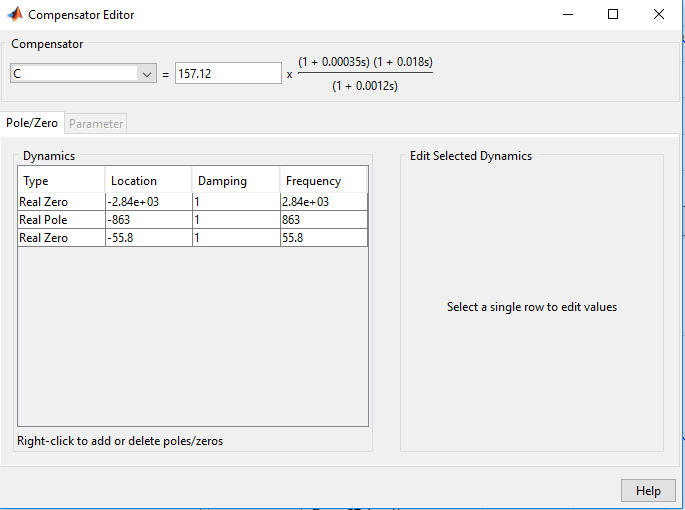
\includegraphics[height=7cm]{img/compensator.PNG}
    \caption{Компенсатор}
    \label{fig:my_label}
\end{figure}
\newpage
Рассмотрим Рис.5 (скорректированная система), можем наблюдать:
\begin{itemize}
    \item Запас устойчивости по фазе: 44.1\degree
    \item Запас устойчивости по амплитуде: 47.9 dB
    \item Амплитуда на рабочая чатота = 44,85 dB
    \item Перерегулированию < 30\%
    \item Cистема является устойчивой и удовлетворяет требованиям по перерегулированию, и по ошибке. 
\end{itemize}
Для оценновании наша система, мы добавили коменсатор на систем управления, настроели график характеристики система:
\begin{enumerate}
    \item ЛАЧХ, ЛФЧХ моделя мотора (рис.6)
    \item ЛАЧХ, ЛФЧХ скорректерованной системы (рис.7)
    \item ЛАЧХ, ЛФЧХ замкнутой системы (рис.8)
    \item Перечщдная характеристики (рис.9)
    \item Погрешность в случае на вход $g(t)=g_m sin(\omega t)$ (рис.10) 
\end{enumerate}
\lstinputlisting[caption = {Код программа (Matlab)}]{ai.m}

\newpage
\begin{landscape}
\begin{figure}[h]
    \centering
    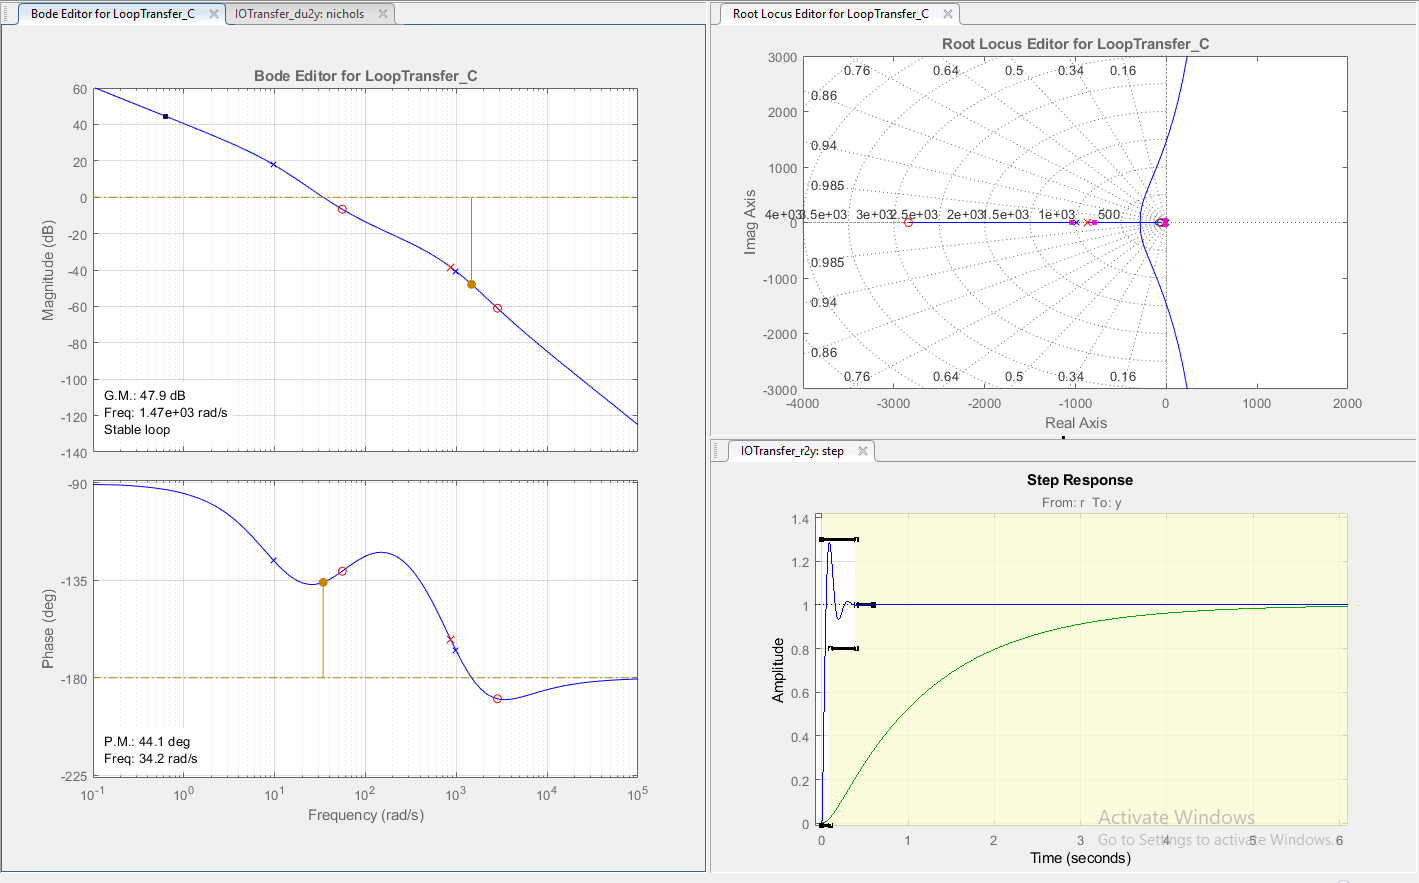
\includegraphics[height=15cm]{img/final.PNG}
    \caption{ЛАЧХ, ЛФЧХ, коренвой годораф скорректированная система}
    \label{fig:my_label}
\end{figure}
\end{landscape}
\newpage

\begin{figure}[h]
    \centering
    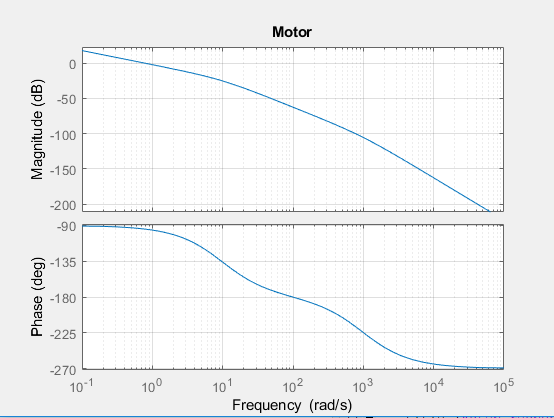
\includegraphics[height=8cm]{img/f1.PNG}
    \caption{ЛАЧХ, ЛФЧХ моделя мотора}
    \label{fig:my_label}
\end{figure}

\begin{figure}[h]
    \centering
    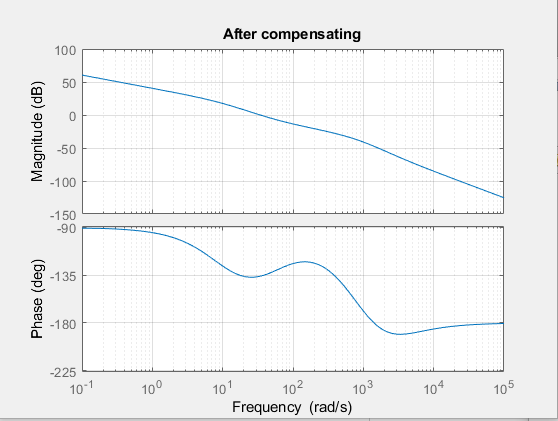
\includegraphics[height=8cm]{img/f2.PNG}
    \caption{ЛАЧХ, ЛФЧХ скорректерованной системы}
    \label{fig:1}
\end{figure}

\begin{figure}[h]
    \centering
    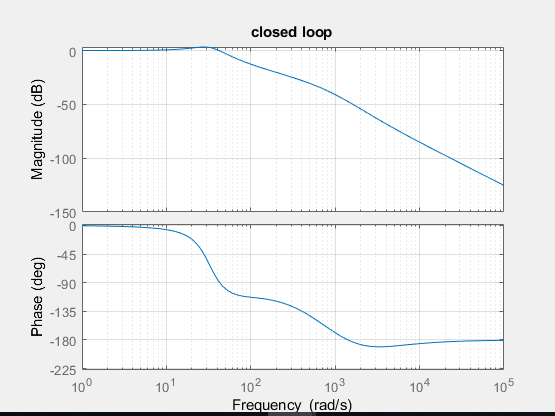
\includegraphics[height=8cm]{img/f3.PNG}
    \caption{ЛАЧХ, ЛФЧХ замкнутой системы}
    \label{fig:23}
\end{figure}

\begin{figure}[h]
    \centering
    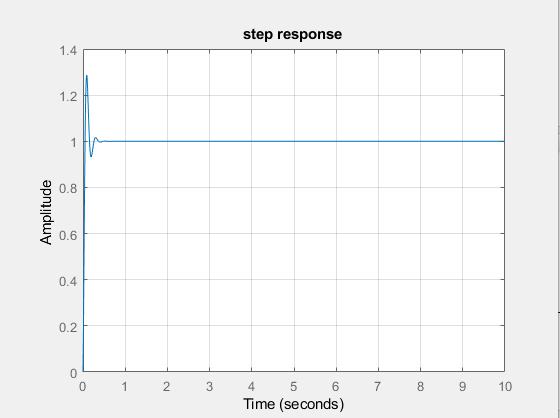
\includegraphics[height=8cm]{img/f4.PNG}
    \caption{Перечщдная характеристики}
    \label{fig:my_label}
\end{figure}

\begin{figure}[h]
    \centering
    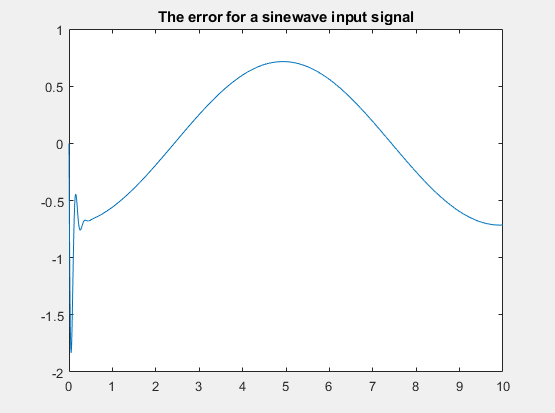
\includegraphics[height=8cm]{img/f5.PNG}
    \caption{Погрешность в случае на вход $g(t)=g_m sin(\omega t)$}
    \label{fig:my_label}
\end{figure}


\end{document}

\usepackage[english,russian]{babel}